%Version 3 December 2023
% See section 11 of the User Manual for version history
%
%%%%%%%%%%%%%%%%%%%%%%%%%%%%%%%%%%%%%%%%%%%%%%%%%%%%%%%%%%%%%%%%%%%%%%
%%                                                                 %%
%% Please do not use \input{...} to include other tex files.       %%
%% Submit your LaTeX manuscript as one .tex document.              %%
%%                                                                 %%
%% All additional figures and files should be attached             %%
%% separately and not embedded in the \TeX\ document itself.       %%
%%                                                                 %%
%%%%%%%%%%%%%%%%%%%%%%%%%%%%%%%%%%%%%%%%%%%%%%%%%%%%%%%%%%%%%%%%%%%%%

%%\documentclass[referee,sn-basic]{sn-jnl}% referee option is meant for double line spacing

%%=======================================================%%
%% to print line numbers in the margin use lineno option %%
%%=======================================================%%

%%\documentclass[lineno,sn-basic]{sn-jnl}% Basic Springer Nature Reference Style/Chemistry Reference Style

%%======================================================%%
%% to compile with pdflatex/xelatex use pdflatex option %%
%%======================================================%%

%%\documentclass[pdflatex,sn-basic]{sn-jnl}% Basic Springer Nature Reference Style/Chemistry Reference Style


%%Note: the following reference styles support Namedate and Numbered referencing. By default the style follows the most common style. To switch between the options you can add or remove “Numbered” in the optional parenthesis. 
%%The option is available for: sn-basic.bst, sn-vancouver.bst, sn-chicago.bst%  
 
%%\documentclass[pdflatex,sn-nature]{sn-jnl}% Style for submissions to Nature Portfolio journals
%%\documentclass[pdflatex,sn-basic]{sn-jnl}% Basic Springer Nature Reference Style/Chemistry Reference Style
\documentclass[pdflatex,sn-mathphys-num]{sn-jnl}% Math and Physical Sciences Numbered Reference Style 
%%\documentclass[pdflatex,sn-mathphys-ay]{sn-jnl}% Math and Physical Sciences Author Year Reference Style
%%\documentclass[pdflatex,sn-aps]{sn-jnl}% American Physical Society (APS) Reference Style
%%\documentclass[pdflatex,sn-vancouver,Numbered]{sn-jnl}% Vancouver Reference Style
%%\documentclass[pdflatex,sn-apa]{sn-jnl}% APA Reference Style 
%%\documentclass[pdflatex,sn-chicago]{sn-jnl}% Chicago-based Humanities Reference Style

%%%% Standard Packages
%%<additional latex packages if required can be included here>

\usepackage{graphicx}%
\usepackage{multirow}%
\usepackage{amsmath,amssymb,amsfonts}%
\usepackage{amsthm}%
\usepackage{mathrsfs}%
\usepackage[title]{appendix}%
\usepackage{xcolor}%
\usepackage{textcomp}%
\usepackage{manyfoot}%
\usepackage{booktabs}%
\usepackage{algorithm}%
\usepackage{algorithmicx}%
\usepackage{algpseudocode}%
\usepackage{listings}%

%% For algorithms...
\algnewcommand\algorithmicforeach{\textbf{for each}}
\algdef{S}[FOR]{ForEach}[1]{\algorithmicforeach\ #1\ \algorithmicdo}
\algnewcommand\algorithmicswitch{\textbf{switch}}
\algnewcommand\algorithmiccase{\textbf{case}}
\algdef{SE}[SWITCH]{Switch}{EndSwitch}[1]{\algorithmicswitch\ #1\ \algorithmicdo}{\algorithmicend\ \algorithmicswitch}
\algdef{SE}[CASE]{Case}{EndCase}[1]{\algorithmiccase\ #1}{\algorithmicend\ \algorithmiccase}
\algtext*{EndSwitch}
\algtext*{EndCase}
%%%%

%%%%%=============================================================================%%%%
%%%%  Remarks: This template is provided to aid authors with the preparation
%%%%  of original research articles intended for submission to journals published 
%%%%  by Springer Nature. The guidance has been prepared in partnership with 
%%%%  production teams to conform to Springer Nature technical requirements. 
%%%%  Editorial and presentation requirements differ among journal portfolios and 
%%%%  research disciplines. You may find sections in this template are irrelevant 
%%%%  to your work and are empowered to omit any such section if allowed by the 
%%%%  journal you intend to submit to. The submission guidelines and policies 
%%%%  of the journal take precedence. A detailed User Manual is available in the 
%%%%  template package for technical guidance.
%%%%%=============================================================================%%%%

%% as per the requirement new theorem styles can be included as shown below
%\theoremstyle{thmstyleone}%
\newtheorem{theorem}{Theorem}%  meant for continuous numbers
%%\newtheorem{theorem}{Theorem}[section]% meant for sectionwise numbers
%% optional argument [theorem] produces theorem numbering sequence instead of independent numbers for Proposition
\newtheorem{proposition}[theorem]{Proposition}% 
%%\newtheorem{proposition}{Proposition}% to get separate numbers for theorem and proposition etc.

%\theoremstyle{thmstyletwo}%
\newtheorem{example}{Example}%
\newtheorem{remark}{Remark}%

%\theoremstyle{thmstylethree}%
\newtheorem{definition}{Definition}%
\newtheorem{lemma}{Lemma}


\raggedbottom
%%\unnumbered% uncomment this for unnumbered level heads

\begin{document}

\title[SDCEL]{On Scalable DCEL Overlay Operations}

%%=============================================================%%
%% GivenName	-> \fnm{Joergen W.}
%% Particle	-> \spfx{van der} -> surname prefix
%% FamilyName	-> \sur{Ploeg}
%% Suffix	-> \sfx{IV}
%% \author*[1,2]{\fnm{Joergen W.} \spfx{van der} \sur{Ploeg} 
%%  \sfx{IV}}\email{iauthor@gmail.com}
%%=============================================================%%

\author*[1]{\fnm{Andres} \sur{Calderon-Romero}}\email{acald013@ucr.edu}

\author[1]{\fnm{Laila} \sur{Abdelhafeez}}\email{labde005@ucr.edu}

\author[2]{\fnm{Goce} \sur{Trajcevski}}\email{gocet25@iastate.edu}

\author[1]{\fnm{Amr} \sur{Magdy}}\email{amr@cs.ucr.edu}

\author[1]{\fnm{Vassilis J.} \sur{Tsotras}}\email{tsotras@cs.ucr.edu}

\affil[1]{\orgdiv{Computer Science Department}, \orgname{University of California}, \orgaddress{\street{900 University Ave}, \city{Riverside}, \postcode{92521}, \state{California}, \country{US}}}
\affil[2]{\orgdiv{Department of Electrical and Computer Engineering}, \orgname{Iowa State University}, \orgaddress{\street{2433 Union Dr}, \city{Ames}, \postcode{50011}, \state{Iowa}, \country{US}}}

%%==================================%%
%% Sample for unstructured abstract %%
%%==================================%%

\abstract{
The Doubly Connected Edge List (DCEL) is an edge-list structure widely used in spatial applications, primarily for planar topological and geometric computations. However, it is also applicable to various types of data, including 3D models and geographic data.
An essential operation is the \textit{overlay operation}, which combines the DCELs of two input polygon layers and can easily support spatial queries on polygons like the intersection, union, and difference between these layers.
However, existing techniques for spatial overlay operations suffer from two main limitations.
First, they fail to handle many large datasets practically used in real applications.
Second, they cannot handle arbitrary spatial lines that practically form polygons, e.g., city blocks, but they are given as a set of scattered lines.
This work proposes a distributed and scalable way to compute the overlay operation and its related supported queries. Our operations also support arbitrary spatial lines through a scalable polygonization process.
We address the issues of efficiently distributing the lines and overlay operators and offer various optimizations that improve performance. Our experiments demonstrate that the proposed scalable solution can efficiently compute the overlay of large real datasets.}

%%================================%%
%% Sample for structured abstract %%
%%================================%%

% \abstract{\textbf{Purpose:} The abstract serves both as a general introduction to the topic and as a brief, non-technical summary of the main results and their implications. The abstract must not include subheadings (unless expressly permitted in the journal's Instructions to Authors), equations or citations. As a guide the abstract should not exceed 200 words. Most journals do not set a hard limit however authors are advised to check the author instructions for the journal they are submitting to.
% 
% \textbf{Methods:} The abstract serves both as a general introduction to the topic and as a brief, non-technical summary of the main results and their implications. The abstract must not include subheadings (unless expressly permitted in the journal's Instructions to Authors), equations or citations. As a guide the abstract should not exceed 200 words. Most journals do not set a hard limit however authors are advised to check the author instructions for the journal they are submitting to.
% 
% \textbf{Results:} The abstract serves both as a general introduction to the topic and as a brief, non-technical summary of the main results and their implications. The abstract must not include subheadings (unless expressly permitted in the journal's Instructions to Authors), equations or citations. As a guide the abstract should not exceed 200 words. Most journals do not set a hard limit however authors are advised to check the author instructions for the journal they are submitting to.
% 
% \textbf{Conclusion:} The abstract serves both as a general introduction to the topic and as a brief, non-technical summary of the main results and their implications. The abstract must not include subheadings (unless expressly permitted in the journal's Instructions to Authors), equations or citations. As a guide the abstract should not exceed 200 words. Most journals do not set a hard limit however authors are advised to check the author instructions for the journal they are submitting to.}

\keywords{Spatial data structures, overlay operator, DCEL}

%%\pacs[JEL Classification]{D8, H51}

%%\pacs[MSC Classification]{35A01, 65L10, 65L12, 65L20, 65L70}

\maketitle

\section{Introduction}

The use of spatial data structures is ubiquitous in many spatial applications, ranging from spatial databases to computational geometry, robotics, and geographic information systems \cite{samet_design_1990}. Spatial data structures have been used to improve the efficiency of various spatial queries, spatial joins, nearest neighbors, Voronoi diagrams, and robot motion planning. Examples include grids \cite{nievergelt_grid_1984}, R-trees \cite{guttman_r-trees_1984, beckmann_r-tree_1990}, and quadtrees \cite{finkel_quadtrees_1974}.  \textit{Edge-list} structures are also typically utilized in applications as topological computations in computational geometry \cite{berg_computational_2008}.

The most commonly used data structure in the edge-list family is the \textit{Doubly Connected Edge List (DCEL)}. A DCEL \cite{muller_finding_1978, preparata_computational_1985} is a data structure that collects topological information for the edges, vertices, and faces contained by a surface in the plane. The DCEL and its components represent a planar subdivision of that surface. In a DCEL, the faces (polygons) represent non-overlapping areas of the subdivision; the edges are boundaries that divide adjacent faces; and the vertices are the point endings between adjacent edges (see Figure \ref{fig:dcel_example}).  In addition to providing geometric and topological information, a DCEL can be enhanced to provide further information. For instance, a DCEL storing a thematic map for vegetation can also store the type and height of the trees around the area \cite{berg_computational_2008}.

\begin{figure}
    \centering
    \includegraphics[width=0.6\linewidth]{chapterSDCEL/dcel_example}
    \caption{Components of the DCEL structure.}\label{fig:dcel_example}
\end{figure}

The DCEL data structure has been used in various applications. For instance, the use of connected edge lists is cardinal to support polygon triangulations and their applications in surveillance (the Art Gallery Problem \cite{chvatal_combinatorial_1975, orourke_art_1987}) and robot motion planning (\cite{berg_computational_2008, chew_convex_1993}). DCELs are also used to perform polygon unions (for example, on printed circuit boards to support the simplification of connected components in an efficient manner \cite{fogel_cgal_2012}) as well as the computation of silhouettes from polyhedra \cite{fogel_cgal_2012, berberich_arrangements_2010} (applied frequently in computer vision and 3D graphics modeling \cite{boguslawski_modelling_2011}).

Edge-list data structures have also been utilized to create thematic \textit{overlay maps}. In this problem, the input contains the DCELs of two polygonal layers, each capturing geospatial information and attribute data for different phenomena, and the output is the DCEL of an overlay structure that combines the two layers into one. In many application areas, such as ecology, economics, and climate change, it is important to be able to join the input layers and match their attributes in order to unveil patterns or anomalies in data that can be highly impacted by location. Several operations can then be easily computed given an overlay; for instance, the user may want to find the \textit{intersection} between the input layers (e.g., corresponding to soil types and evapotranspiration of plants), identify their \textit{difference} (or symmetric difference), or create their \textit{union}. 

Spatial databases use spatial indexes (R-tree \cite{guttman_r-trees_1984, beckmann_r-tree_1990}) to store and query polygons. Such methods use the \textit{filter and refine} approach where a complex polygon is abstracted by its Minimum Bounding Rectangle (MBR); this MBR is then inserted in the R-tree index. Finding the intersection between two polygon layers, each indexed by a separate R-tree, is then reduced to finding the pairs of MBRs from the two indexes that intersect (filter part). This is followed by the refine part, which, given two MBRs that intersect, needs to compute the actual intersections between all the polygons these two MBRs contain. While MBR intersection is simple, computing the intersection between a pair of complex real-life polygons is a rather expensive operation (a typical 2020 US census tract is a polygon with hundreds of edges).  Moreover, using DCELs for overlay operations offers the additional advantage that the result is also a DCEL, which can be directly used for subsequent operations. For example, one may want to create an overlay between the intersection of two layers with another layer, and so on.

Even though the DCEL has important advantages for implementing overlay operations, current approaches are sequential in nature. This is problematic, considering layers with thousands of polygons. For example, the layer representing the 2020 US census tracts contains around 72K polygons; the execution for computing the overlay over such a large file crashed on a stock laptop. To the best of our knowledge, there is no scalable solution for computing overlays over DCEL layers.

%% Extension
% In addition to the scalability issue, it is common in some applications that spatial polygons are provided in the form of scattered line segments, e.g., a set of road segments that form city blocks.  Such data can be very large and appear in applications in urban planning, geo-targeted advertising, economic and demographic studies, etc.  Yet, existing polygon overlay techniques cannot handle them directly at scale.  In that setting, extracting the DCEL subdivision's faces (polygons) is not straightforward.  To generate all of a subdivision's faces, the DCEL constructor must invoke a scalable \textit{polygonization} procedure, which extracts all closed polygons formed by a collection of planar line segments in a subdivision.

This chapter describes the design and implementation of a \textit{scalable} and \textit{distributed} approach to compute the overlay between two DCEL layers. We first present a partitioning strategy that guarantees that each partition collects the required data from each layer DCEL to work independently, thus minimizing duplication and transmission costs over 2D polygons. In addition, we present a merging procedure that collects all partition results and consolidates them in the final combined DCEL.

%% Extension
%Furthermore, we extend the overlay method to support input polygons in scattered line segments form by integrating a scalable and distributed polygon extraction approach.  Our solutions have been implemented in a parallel framework (i.e., Apache Spark).

Implementing a distributed overlay DCEL creates novel problems. First, there are potential challenges that are not present in the sequential DCEL execution. For example, the implementation should consider \textit{holes}, which could lay on different partitions, and they need to be connected with their components residing in other partitions so as not to compromise the combined DCEL's correctness.

%% Extension
%It should also consider the \textit{dangle} and \textit{cut edges} resulting from the polygonization process and their intersection with other polygon layers.

Secondly, once a distributed overlay DCEL has been built, it must support a set of binary overlay operators (namely \textit{union, intersection, difference} and \textit{symmetric difference}) in a transparent manner.  That is, such operators should take advantage of the scalability of the overlay DCEL and be able to run also in a parallel fashion. Additionally, users should be able to apply the various operators multiple times without rebuilding the overlay DCEL data structure.  

%% Extension
%This chapter extends the previous work in \cite{calderon_scalable_2023}. The main new contributions are summarized as follows. First, we introduce a new spatial partitioner, based on the kd-tree partitioning strategy, for constructing overlay  DCELs (section \ref{sec:kdtreestrategy}). Since it better utilizes the data  distributions in optimizing DCEL partitions, it leads to noticeably improved performance. The new partitioning strategy contrasts with the original strategy that employed space-partitioning techniques based on quadtrees. Second, we enable overlay DCELs to take scattered and noisy line segments as input instead of being limited to clean polygon data.  This builds on the work on scalable polygonization in \cite{abdelhafeez_ddcel_2023} to enable overlays of real datasets that consist of massive sets of line segments that cannot currently be handled by any existing technique. We also provide additional experiments, to quantify the benefits of the kd-tree based strategy, as well as the performance on the datasets with large volumes of line segments.

The rest of this chapter is organized as follows. Section \ref{sec:related} presents related work, while Section \ref{sec:prelim} discusses the basics of DCEL and the sequential algorithm. In Section \ref{sec:methods}, we present the partitioning schemes that enable parallel implementation of the overlay computation among DCEL layers; we also discuss the challenges presented in the DCEL computations by distributing the data and how to solve them efficiently. Two important optimizations are introduced in Section \ref{sec:alternative_methods}. Finally, an extensive experimental evaluation appears in Section \ref{sec:experiments}.

%% Extension
%Section~\ref{sec:polygonization} details the polygon extraction process for line input adaptation. It also extends the overlay method by supporting the overlay of dangle and cut edges.

\vspace{-5pt}
\section{Related Work}
\label{sec:related}
The fundamentals of the DCEL data structure were introduced in the seminal paper by Muller and Preparata  \cite{muller_finding_1978}. The advantages of DCELs are highlighted in \cite{preparata_computational_1985, berg_computational_2008}.
%, including the ability to capture topological information and support various overlay operators 
Examples of using DCELs for diverse applications appear in\cite{barequet_dcel_1998, boltcheva_topological-based_2020, freiseisen_colored_1998}. 
Once the overlay DCEL is created by combining two layers,  
%A DCEL can be constructed in $\mathcal{O}(n log(n))$ time using $\mathcal{O}(n)$ additional memory where $n$ is the number of vertices in the input layer \cite{freiseisen_colored_1998}. 
%Given the overlay DCEL of two layers, 
overlay operators like union, difference etc., can be computed in linear time to the number of faces in their overlay \cite{freiseisen_colored_1998}. 

Currently, few sequential implementations are available: LEDA
%\footnote{\url{https://www.algorithmic-solutions.com/}} 
\cite{mehlhorn_leda_1995}, Holmes3D
%\footnote{\url{http://www.holmes3d.net/graphics/}} 
\cite{holmes_dcel_2021} and CGAL
%\footnote{\url{https://www.cgal.org/}} 
\cite{fogel_cgal_2012}.  Among them CGAL is an open-source project widely used for computational geometry research. 
%It offers a wide-ranging number of packages and modules to support diverse topics including a solid support for DCEL construction.
To the best of our knowledge, there is no scalable implementation for the computation of overlay DCEL.

While there is a lot of work on using spatial access methods to support spatial joins, intersections, unions etc. in a parallel way (using clusters, multicores or GPUs), \cite{challa_dd-rtree_2016, sabek_spatial_2017, li_scalable_2019, franklin_data_2018, magalhaes_fast_2015, puri_efficient_2013, puri_mapreduce_2013} these approaches are different in two ways: (i) after the index filtering, they need a time-consuming refine phase where the operator (union, intersection etc.) has to be applied on each pair of (typically) complex spatial objects; (ii) if the operator changes, we need to run the filter/refine phases from scratch (in contrast, the same overlay DCEL can be used to run all operators.)

%Although there is not reference to scalable DCEL implementations, other dynamic parallel data structures has been described   However, spatial indexes and spatial joins could support overlay operators in certain way but just for an individual operator at a time. 

%Another works present parallel map overlay algorithms whose focus on GPU and multi-core architecture \cite{franklin_data_2018, magalhaes_fast_2015, puri_efficient_2013, puri_mapreduce_2013}.  Most of them use scan line algorithms to partition the edges and hierarchical tree structures (such as octree or rtree) to partition the input data. However, they support only the intersection overlay operator. Even though, these works focus on solutions aim to multi-core architectures or GPGPU models which scalability can be affected by very large datasets.  In addition, implementations over the traditional multi-core ecosystem could not take total advantage of modern distributed memory frameworks such as Apache Spark.



\section{Preliminaries}

\begin{table} %\label{tab:records}
    \ssp
    \begin{minipage}{0.5\textwidth}
        \small
        \centering
        \caption{Vertex records.}\label{tab:vertices}
        \begin{tabular}{c c c}
            \toprule
            vertex & coordinates & incident edge \\
            \midrule
            a      & (0,2)  & $\vec{ba}$ \\
            b      & (2,0)  & $\vec{db}$ \\
            c      & (2,4)  & $\vec{dc}$ \\
            \vdots & \vdots & \vdots     \\
            \bottomrule
        \end{tabular}
    \end{minipage}\hfill % maximize the horizontal separation
    \begin{minipage}{0.5\textwidth}
        \small
        \centering
        \caption{Face records.}\label{tab:faces}
        \begin{tabular}{c c c}
            \toprule
                & boundary  & hole\\
            face & edge      & list\\
            \midrule
            $f_1$ & $\vec{ab}$ & $nil$ \\
            $f_2$ & $\vec{fe}$ & $nil$ \\
            $f_3$ & $nil$      & $nil$ \\
            \bottomrule
        \end{tabular}
    \end{minipage}
\end{table}

\begin{table}
    \ssp
    \small
    \centering
    \caption{Half-edge records.}\label{tab:hedges}
    \begin{tabular}{c c c c c c} 
        \toprule
        half-edge & origin & face & twin & next & prev \\
        \midrule
        $\vec{fe}$ & f & $f_2$  & $\vec{ef}$ & $\vec{ec}$ & $\vec{df}$ \\
        $\vec{ca}$ & c & $f_1$  & $\vec{ac}$ & $\vec{ab}$ & $\vec{dc}$ \\
        $\vec{db}$ & d & $f_3$  & $\vec{bd}$ & $\vec{ba}$ & $\vec{fd}$ \\
        \vdots     & \vdots & \vdots & \vdots     & \vdots     & \vdots     \\
        \bottomrule
    \end{tabular}
\end{table}

\label{sec:prelim}

The DCEL \cite{muller_finding_1978} structure is used to represent an embedding of a planar subdivision in the plane. It provides efficient manipulation of the geometric and topological features of spatial objects (polygons, lines and points) using \textit{faces}, \textit{edges} and \textit{vertices} respectively.  
A DCEL uses three tables (relations) to store records for the faces, edges and vertices, respectively. 
An important characteristic is that all these records are defined using edges as the main component (thus termed as an edge-based structure). 
Examples appear in Tables \ref{tab:vertices}-\ref{tab:hedges} below, following the subdivision depicted in Figure \ref{fig:dcel_example}.

An edge corresponds to a straight line segment, shared by two adjacent faces (polygons).
Each of these two faces will use this edge in its description; to distinguish, each edge has two \textit{half-edges}, one for each orientation (direction).
It is important to note that half-edges are oriented counter clockwise inside each face (Figure \ref{fig:dcel_example}).
A half-edge is thus defined by its two vertices, one called the \textit{origin} vertex and the other the \textit{target} vertex, clearly specifying the half-edge's orientation (origin to target).
Each half-edge record contains references to its origin vertex, its face, its \textit{twin} half-edge, as well as the next and previous half-edges (using the orientation of its face); see Table \ref{tab:hedges}. These references are used as keys to the tables that contain the referred attributes. 

Figure \ref{fig:dcel_example} shows half-edge $\overrightarrow{fe}$, its \textit{twin($\overrightarrow{fe}$)} (which is half-edge $\overrightarrow{ef}$), the \textit{next($\overrightarrow{fe}$)} (half-edge $\overrightarrow{ec}$) and the \textit{prev($\overrightarrow{fe}$)} (half-edge $\overrightarrow{df}$). Note the counter clockwise direction used by the half-edges comprising face $f_2$. 
The \textit{incidentFace} of a half-edge corresponds to the face that this edge belongs to (for example \textit{incidentFace}($\overrightarrow{fe}$) is face $f_2$).

Each vertex corresponds to a record in the vertex table (see Table \ref{tab:vertices}) that contains its coordinates as well as one of its incident half-edges. An incident half-edge is one whose target is this vertex. Any of the incident edges can be used; the rest of a vertex's incident half-edges can be found easily following next and twin half-edges.

Finally, each record in the faces table contains one of the face's half edges to describe the polygon's outer boundary (following this face's orientation); see Table \ref{tab:faces}. 
All other half-edges for this face's boundary can be easily retrieved following next half-edges in orientation order.
In addition to regular faces, there is one face that covers the area outside all faces; it is called the  \textit{unbounded} face (face $f_3$ in Figure \ref{fig:dcel_example}). 
Since $f_3$ has no boundary, its boundary edge is set to \textit{nil} in Table \ref{tab:faces}.
Note, that polygons can contain one or more \textit{holes} (a hole is an area inside the polygon that does not belong to it). 
Each such hole is itself described by one of its half-edges; this information is stored as a list attribute (hole list) in the faces table where each element of the list is the half-edge's id which describe the hole. Note that in Table \ref{tab:faces} this list is empty as there are no holes in any of the faces in the example of Figure \ref{fig:dcel_example}. 

An important advantage with the DCEL structure is that a user can combine two DCELs from different layers over the same area (e.g. the census tracks from two
different years) and compute their \textit{overlay} which is a DCEL structure that combines the two layers into one. Other operators like the intersection,
difference etc. can then be computed from the overlay very efficiently.
Given two DCEL layers $S_1$ and $S_2$, a face $f$ appears in their overlay  $OVL(S_1, S_2)$ if and only if there are faces $f_1$ in $S_1$ and $f_2$ in $S_2$ such that $f$ is a maximal connected subset of $f1 \cap f2$ \cite{berg_computational_2008}.  
This property implies that the overlay $OVL(S_1, S_2)$ can be constructed using the half-edges from $S_1$ and $S_2$ . 

The sequential algorithm \cite{fogel_cgal_2012} to construct the overlay between two DCELs first extracts the half-edge segments from the half-edge tables and then finds intersection points between half-edges from the two layers (using a sweep line approach) \cite{berg_computational_2008}. 
The intersection points found will become new vertices of the resulting overlay. 
If an existing half-edge contains an intersection point it is split into two new half-edges. 
Using the list of outgoing and incoming half-edges for the newly added vertices (intersection points) the algorithm can compute the attributes for the records of the new half-edges. For example, the list of outgoing and incoming half-edges at each new vertex will be used to update the next, previous and twin pointers. Finally, records for faces and vertices tables are also updated with the new information. 

\begin{figure}
    \centering
    \includegraphics[width=\linewidth]{figures/dcel_seq/dcel2}
    \caption{Sequential computations of an overlay of two DCEL layers.}\label{fig:dcel_seq}
\end{figure}

Figure \ref{fig:dcel_seq} illustrates an example for computing the overlay between two DCEL layers with one face each ($A_1$ and $B_1$ respectively), that overlap over the same area. First, intersection points are found and create new vertices in the overlay (red vertices $c_1$ and $c_2$). Finally, new half edges are created around these new vertices. 
As a result, face $A_1$ is modified (to an L-shaped boundary) as does face $B_1$, while a new face $A_1B_1$ is created. 
Since this new face is the intersection of the boundaries of $A_1$ and $B_1$, its label contains the concatenation of both face labels. 
By convention \cite{berg_computational_2008}, even though $A_1$ changes its shape, it does not change its label since its new shape is created by its intersection with the unbounded face of $B_1$; similarly the new shape of $B_1$ maintains its original label. 
These labels are crucial for the creation of the overlay (and the operators it supports) as they are used to identify which polygons overlap an existing face.

Once the overlay structure of two DCELs is computed, queries like their intersection, union, difference etc. (Figure \ref{fig:dcel_operators}) can be performed in linear time to the number of faces in the overlay. 
The space requirement for the overlay structure remains linear to the number of vertices, edges and faces.  
Since an overlay is itself a DCEL, it can support the traditional DCEL operations (e.g., find the boundary of a face, access a face from an adjacent one, visit all the edges around a vertex, etc.)

\begin{figure*}
    \centering
    \includegraphics[width=0.9\textwidth]{figures/dcel_operators/dcel_operators.pdf}
    \caption{Examples of overlay operators supported by DCEL; results are shown in gray.}
    \label{fig:dcel_operators}
\end{figure*}

\section{Scalable Overlay Construction} \label{sec:methods}

The overlay computation depends on the size of the input DCELs and the size of the resulting overlay.
The DCEL of a planar subdivision $S_1$ has size $O(n_1)$ where $n_1$ = $\Sigma (vertices_1 + edges_1 + faces_1$).
The sequential algorithm constructing the overlay of $S_1$ and $S_2$ takes $O(n \log n + k \log n)$ time, where $n = n_1 + n_2$ and $k$ is the size of their
overlay.
Note that $k$ depends on how many intersections occur between the input DCELs, which can be very large \cite{berg_computational_2008}. 

While the sequential algorithm is efficient with small DCEL layers, it suffers when the input layers are large and have many intersections. 
For example, creating the overlay between the DCELs of two census tracks (from years 2000 and 2010) from California (each with 7K-8K polygons and 2.7M-2.9M edges) took about 800sec on an Intel Xeon CPU at 1.70GHz  with 2GB of memory (see Section  \ref{sec:experiments}).
With DCELs corresponding to the whole US, the algorithm crashed. 

Nevertheless, the overlay computation can take advantage of partitioning (and thus parallelism), by observing that the edges in a given area of one input layer, can only intersect with edges from the same area in the other input layer. 
One can thus spatially partition the two input DCELs using a spatial index (or grid) and then compute the overlay within each cell; such computations are independent and can be performed in parallel. 
While this is a high level view of our scalable approach, there are various challenges, including how to deal with edges that cross cells, how to manage the extra complexity introduced by \textit{orphan} holes (i.e., when holes and their polygons are in different cells), how and where to combine partition overlays into a global overlay, as well as how to balance the computation if one layer is much larger than the other. 

\subsection{Partition Strategy} \label{sec:strategy}
The main idea of the partition strategy is to split the area covered by the input layers into non-overlapping cells which could then be processed independently.  
One could use a simple grid to divide the area but our early experiments showed that such approach would result in unbalanced cells (in number of edges) which affects performance. 
In the rest we assume that the partitioning is performed using a quadtree index which adapts to skewed spatial distributions and helps to assign a similar number of edges to each cell. 

The overall approach can be summarized in the following steps: (i) Partition the input layers into the index cells and build local DCEL representations of them at each cell; and (ii) Compute the overlay of the DCELs at each cell.  
Overlay operators and other functions can be run over the local overlays and then local results are collected to generate the final answer.  

Note that each input layer is given as a sequence of polygon edges, where each edge record contains the coordinates of the edge's vertices (origin and target vertex) as well as the polygon id and a hole id in the case that an edge belongs to a hole inside of a polygon. We assume there are not overlapping or stacked polygons in the dataset.  To quickly build the partitioning quadtree structure we take a sample from the edges of each layer (1\% of the total number of edges in that layer). After the quadtree is created, we use its leaf nodes as the partitioning cells for each layer. 
Each input layer file is then read from disk and \textit{all} of its edges are inserted to the appropriate cells of the partitioning structure.

For this approach to work, it is important that each cell can compute its two DCELs independently. 
Note that an edge can be fully contained in a cell, or it can intersect the cell's boundary.
In the second case, we copy this edge to all cells that it intersects, but within each cell, we use the part of the edge that lies fully inside the cell. 
Figure \ref{fig:partition_strategy} shows an example, where there are 4 cells and two edges of the upper polygon from layer A cross the cell borders. Such edges are clipped at the cell borders, introducing new edges (e.g. edges $\alpha^{\prime}$ and $\alpha^{\prime \prime}$ in the Figure \ref{fig:partition_strategy}).  
Similarly, a polygon that crosses over a cell is clipped to the cell by introducing \textit{\textbf{artificial}} edges on the cell's border (see face $A_2$ in cell 3 of Figure \ref{fig:partition_strategy}). 
Such artificial edges are shown in red in the figure. 
This allows to create a smaller polygon that is contained within each cell. For example polygon $A_2$ is clipped into four smaller polygons as it overlaps all four cells. 
The clipping of edges and polygons ensures that each cell has all needed information to complete its DCEL computations. 
As such computations can be performed independently, they are sent to different compute nodes to be processed in parallel.  The assignment is delegate to the distributed framework (i.e. Apache Spark).  

\begin{figure*}
    \centering
    \includegraphics[width=0.65\textwidth]{figures/partition_schema/PolygonsParted}
    \caption{Partitioning example using input layers A and B over four cells.}\label{fig:partition_strategy}
\end{figure*}

Once a cell is assigned to a node, the sequential algorithm is used to create a DCEL for each layer (using the cell edges from that layer and any artificial edges, vertices and faces created by the clipping procedures above) and then compute the corresponding (local) overlay for this cell. 
Using the example from Figure \ref{fig:partition_strategy}, Figure \ref{fig:overlay_partition} depicts an overview of the process for creating a local overlay DCEL inside cell 2.  
Similarly, Figure \ref{fig:distributed_dcel} shows all local overlay DCELs computed at each cell (again, artificial edges are shown in red). 

Nevertheless, the partitioning can create two problems (not present in the sequential environment) that need to be addressed. 
The first is the case where a cell is empty, that is, it does not intersect with (or contain) any regular edge from neither layer. A regular edge is one that is not part of a hole.
This empty cell does not contain any label and thus we do not know which face it may belongs to. We term this as the \textbf{\textit{orphan cell}} problem.
An example is shown in Figure \ref{fig:emptycellexample} which depicts a face (from one of the input layers) whose boundary goes over many quadtree cells; orphan cells are shown in grey. 

Note that an orphan cell may contain a hole (see Figure \ref{fig:emptycellexample}). 
In this case the original label of the face where the hole belongs (and reported in the hole's edges) may have changed during the overlay computation (because it overlapped with a face from the other layer). 
However, this new label has not been propagated to the hole edges.
We term this as the \textbf{\textit{orphan hole}} problem.
While for simplicity we focus in the case where a hole is within one orphan cell, in the general case, a hole can split among many such cells.

The issue with both `orphan' problems is the missing labels. Below we propose an algorithm that correctly labels an orphan cell. If this cell contains a hole, the new label is used to update the hole edges as well. 

\begin{figure}
    \centering
    \includegraphics[width=0.9\linewidth]{figures/overlay_partition/overlay_partition.pdf}
    \caption{Local overlay DCEL for cell 2.}\label{fig:overlay_partition}
\end{figure}

\begin{figure}
    \centering
    \includegraphics[width=0.6\linewidth]{figures/distributed_dcel/distributed_dcel.pdf}    
    \caption{Result of the local overlay DCEL computations.}\label{fig:distributed_dcel}
\end{figure}

\begin{figure*}
    \centering
    \subfloat[]{\includegraphics[page=1, width=0.23\textwidth]{figures/empty_cells/emptycells2}\label{fig:orphan1}}
    \subfloat[]{\includegraphics[page=1, width=0.22\textwidth]{figures/empty_cells/example}\label{fig:orphan2}}
    \subfloat[]{\includegraphics[page=2, width=0.22\textwidth]{figures/empty_cells/example}}
    \subfloat[]{\includegraphics[page=3, width=0.22\textwidth]{figures/empty_cells/example}}
    
    \caption{(a) Empty cell and hole examples; (b)-(c)-(d) show three iterations of the proposed solution.} 
    \label{fig:emptycellexample}
\end{figure*}

\subsection{Labeling Orphan Cells and Holes} \label{sec:anomalies}

To find the label of an orphan cell we propose an algorithm that recursively searches the space around the orphan cell until it identifies a nearby cell which contains edge(s) of the face that contains the orphan cell and thus acquire the appropriate label information. 
This search is accommodated by the quadtree index. 
Two observations are in order: (1) each cell is a leaf of the quadtree index (by construction), and (2) each cell has a unique id created by the way this cell was created; this id effectively provides the \textit{lineage} (unique path) from the quadtree root to this leaf. 
Recall that the root has four possible children (typically numbered as 0,1,2,3 corresponding to the four children NW, NE, SW and SE). 
The lineage is the sequence of these numbers in the path to the leaf.
For example, the lineage for the shaded orphan cell in Figure \ref{fig:orphan1} is 03.
Further, note that the quadtree is an unbalanced structure, having more deep leaves where there are more edges. Thus higher leaves correspond to larger areas and deeper leaves to smaller areas (since a cell split is created when a cell has more edges than a threshold). 

After identifying an orphan cell, the question is where to search for a cell that will contain an edge. The following Lemma applies:

\begin{lemma}\label{lem:cells}
Given an orphan cell, one of its siblings at the same quadtree level  must contain a regular edge (directly or in its subtree). 
\end{lemma}

This lemma arises from the simple observation that if all three siblings of an orphan cell are empty then there is no reason for the quadtree to make this split and create these four siblings. 
Based on the lemma, we know that one of the three siblings of the orphan cell can lead us to a cell with an edge. 
However, these siblings may not be cells (leaves). 
Instead of searching each one of them in the quadtree until we reach their leaves, we want a way to quickly reach their leaves. 
To do so, we pick the centroid point of the orphan cell's parent (which is also one of the corners of the orphan cell). 
For example, the parent centroid for the orphan cell 03 is the green point in Figure \ref{fig:orphan2}.
We then query the quadtree to identify which cells (leaves; one from each sibling) contain this point. 
We check these cells if they contain an edge; if we find such a cell we stop (and use the label in that cell).
If all three cells are orphans, we need to continue the search. This is the case in Figure \ref{fig:orphan2}, where all three cells (green in the figure) are also orphan.

The algorithm has to pick one of them as the current orphan cell and repeat the process recursively. One can use different heuristics. 
Below we consider the case where we use the deepest cell (i.e. the one with the longest lineage) among the three. This is because, we expect that this will lead us to the denser areas of the quadtree index, where there is more chance to find cells with edges.
Figure \ref{fig:emptycellexample} shows a three-iteration run of the algorithm.

During the search process we keep any orphan cells we discover; after a cell with an edge (non-orphan cell) is found, the algorithm stops and labels the original orphan cell and any other orphan cells retrieved in the search with the label found in the non-orphan cell.
Note that if the non-orphan cell contains many labels (because different faces pass through it), we assign the label of the face that contains the original centroid.
The pseudocode of the search process can be seen at Algorithms \ref{alg:one} and \ref{alg:two}.  

Another heuristic we used (not described here) is to follow the highest among the three orphan cells (the one with the shorter lineage) since this has larger area and will thus help us cover more empty space and possibly reach the border of the face faster.

\begin{algorithm}
    \ssp
    \small
    \caption{\textsc{getNextCellWithEdges} algorithm}\label{alg:one}
    \begin{algorithmic}[1]
    \Require a quadtree $\mathcal Q$ and a list of orphan cells $\mathcal M$.
    \Function{ getNextCellWithEdges }{ $\mathcal Q$, $\mathcal M$ }
        \State $\mathcal C \gets $ list of orphan cells in $\mathcal M$
        \ForEach{ $orphanCell$ in $\mathcal C $ }
            \State initialize $cellList$ with $orphanCell$
            \State $nextCellWithEdges \gets null$
            \State $referenceCorner \gets null$
            \State $done \gets false$
            \While{ not $done$ }
                \State $c \gets $ last cell in $cellList$
                \State $cells, corner \gets \textsc{getCellsAtCorner}(\mathcal Q, c)$
                %\Comment{ return 3 cells and the reference corner }
                \ForEach{$cell$ in $cells$}
                    \State $nedges \gets$ get edge count of $cell$ in $\mathcal M$
                    \If{ $nedges > 0$ }
                        \State $nextCellWithEdges \gets cell$
                        \State $referenceCorner \gets corner$
                        \State $done \gets true$
                    \Else
                        \State add $cell$ to $cellList$
                    \EndIf
                \EndFor
            \EndWhile
            \ForEach{ $cell$ in $cellList$ }
                \State \textbf{output}($cell$, \\
                \hspace{2.5cm} $nextCellWithEdges$, $referenceCorner$)
                \State remove $cell$ from $\mathcal C$
            \EndFor
        \EndFor
    \EndFunction
    \end{algorithmic}
\end{algorithm}

\begin{algorithm}
    \ssp
    \small
    \caption{\textsc{getCellsAtCorner} algorithm}\label{alg:two}
    \begin{algorithmic}[1]
    \Require a quadtree with cell envelopes $\mathcal Q$ and a cell $c$.
    \Function{ getCellsInCorner }{ $\mathcal Q$, $c$ }
        \State $region \gets $ quadrant region of $c$ in $c.parent$
        \Switch{ $region$ }
            \Case{ `SW' }
                \State $corner \gets$ left bottom corner of $c.envelope$
            \EndCase
            \Case{ `SE' }
                \State $corner \gets$ right bottom corner of $c.envelope$
            \EndCase
            \Case{ `NW' }
                \State $corner \gets$ left upper corner of $c.envelope$
            \EndCase
            \Case{ `NE' }
                \State $corner \gets$ right upper corner of $c.envelope$
            \EndCase
        \EndSwitch
        \State $cells \gets$ cells which intersect $corner$ in $\mathcal Q$
        \State $cells \gets cells - c$
        %\Comment{ Remove the current cell from the intersected cells }
        \State $cells \gets$ sort $cells$ on basis of their depth
        %\Comment{ using $cell.lineage$ }
        \State \Return{ ($cells$, $corner$) }
    \EndFunction
    \end{algorithmic}
\end{algorithm}

% \begin{algorithm}
%     \caption{\textsc{getNextCellWithEdges} algorithm}\label{alg:one}
%
%     \SetKwProg{Function}{function}{:}{end}
%     \KwIn{a quadtree $\mathcal Q$ and a list of cells $\mathcal M$.}
%     \Function{\textsc{getNextCellWithEdges}($\mathcal Q$,$\mathcal M$)}{
%         $\mathcal C \gets $ orphan cells in $\mathcal M$\\
%          \ForEach{$orphanCell$ in $\mathcal C$}{
%             initialize $cellList$ with $orphanCell$ \\
%             $nextCellWithEdges \gets nil$ \\
%             $referenceCorner \gets nil$ \\
%             $done \gets false$ \\
%             \While{ $\neg done$}{
%                 $c \gets $ last cell in $cellList$ \\
%                 $cells, corner \gets \textsc{getCellsAtCorner}(\mathcal Q, c)$ \\
%                 \ForEach{$cell$ in $cells$}{
%                     $nedges \gets$ get edge count of $cell$ in $\mathcal M$ \\
%                     \eIf{ $nedges > 0$ }{
%                         $nextCellWithEdges \gets cell$ \\
%                         $referenceCorner \gets corner$ \\
%                         $done \gets true$ \\
%                     }{
%                         add $cell$ to $cellList$ \\
%                     }
%                 }
%             }
%             \ForEach{ $cell$ in $cellList$ }{
%                 \textbf{output}($cell$,$nextCellWithEdges$, $referenceCorner$) \\
%                 remove $cell$ from $\mathcal C$ \\
%             }
%         }
%     }
% \end{algorithm}
%
% \begin{algorithm}
%     \small
%     \caption{\textsc{getCellsAtCorner} algorithm}\label{alg:two}
%
%     \SetKwProg{Function}{function}{:}{end}
%     \KwIn{a quadtree with cell envelopes $\mathcal Q$ and a cell $c$.}
%     \Function{ \textsc{getCellsAtCorner}($\mathcal Q$, $c$) }{
%         $region \gets $ quadrant region of $c$ in $c.parent$ \\
%         \Switch{ $region$ }{
%             \uCase{ `SW' }{
%                 $corner \gets$ left bottom corner of $c.envelope$ \\
%             }
%             \uCase{ `SE' }{
%                 $corner \gets$ right bottom corner of $c.envelope$ \\
%             }
%             \uCase{ `NW' }{
%                 $corner \gets$ left upper corner of $c.envelope$ \\
%             }
%             \uCase{ `NE' }{
%                 $corner \gets$ right upper corner of $c.envelope$ \\
%             }
%         }
%         $cells \gets$ cells which intersect $corner$ in $\mathcal Q$ \\
%         $cells \gets cells - c$ \\
%         $cells \gets$ sort $cells$ on basis of their depth \\
%
%         \Return{ ($cells$, $corner$) }
%     }
% \end{algorithm}

\subsection{Answering global overlay queries} \label{sec:reduce}

Using the local overlay DCELs we can easily compute the global overlay DCEL; for that we simply need a reduce phase (described below) to remove artificial edges (and concatenate split edges) from all the faces. Using the local overlay DCELs we can also compute (in a scalable way) global operators like intersection, difference, symmetric difference, etc. For these operators there is first a map phase that computes the specific operator on each local DCEL, followed by a reduce phase to remove artificial edges/added vertices.
Figure \ref{fig:overlay_operator} shows how the intersection overlay operator ($A \cap B$) is computed, starting with the local DCELs for 4 cells (Figure \ref{fig:overlay_operatora}).
First each cell computes the intersection using its local overlay DCEL (Figure \ref{fig:overlay_operatorb}).
This is a simple map operation as we just need to identify overlay faces that contain both labels (from layer A and layer B).
Each cell can then report every such face that does not include any artificial edges (like face $A_1B_1$ in Figure \ref{fig:overlay_operatorb}); note that these faces are fully included in the cell. 

Using a reduce phase, the remaining faces are sent to a master node, in our implementation it would be the driver node of the spark application, that will: (i) remove the artificial edges (shown red in the figure), and (ii) concatenate edges that were split because they were crossing cell borders.
This is done by pairing faces with the same label and concatenating their geometries by removing the artificial edges and vertices added during the partition stage (for example the two faces with label $A_2B_1$ from two different cells in Figure \ref{fig:overlay_operatorb} were combined into one face in Figure \ref{fig:overlay_operatorc} while the extra vertex was also removed).
In section ~\ref{sec:optimizing} we discuss techniques to optimize the reduce process of combining faces.  

For symmetric difference ($A \bigtriangleup B$), the map phase filters faces whose label is a single layer (A or B).  
For the difference ($A \setminus B$), it filters faces with label A. For union ($A \cup B$), all faces in the overlay structure are retrieved. 

\begin{figure}
    \centering
    \subfloat[\label{fig:overlay_operatora}]{\includegraphics[width=0.32\linewidth]{figures/overlay_operator/overlay}}
    \hfill
    \subfloat[\label{fig:overlay_operatorb}]{\includegraphics[width=0.32\linewidth]{figures/overlay_operator/operator}}
    \hfill
    \subfloat[\label{fig:overlay_operatorc}]{\includegraphics[width=0.32\linewidth]{figures/overlay_operator/reduce}}
    \caption{Example of an overlay operator querying the distributed DCEL.} \label{fig:overlay_operator}
\end{figure}

\section{Overlay evaluation optimizations}\label{sec:alternative_methods}
\subsection{Optimizations for faces expanding cells}\label{sec:optimizing}

The (naive) reduce phase described above has the potential for a bottleneck since all faces (which can be a very large number) are sent to one node.
One observation is that faces from different cells that are concatenated are in contiguous cells. 
This implies that faces from a particular cell will be combined with faces from neighboring cells.
We will use this spatial proximity property to reduce the overhead in the central node.


We thus propose an alternative, where an intermediate reduce processing step is introduced.
In particular, the user can specify a level in the quadtree structure (measured as the depth from the root) that can be used to combine cells together. 
Given level \textit{i}, the quadtree nodes in that level (at most $4^i$) will serve as intermediate reducers, collecting the faces from all the cells below that node. (Note: level 0 corresponds to the root, which is the naive method where all the cells are sent to one node).

By introducing this intermediate step it is expected that much of the reduce work can be distributed in a larger number of nodes.
Nevertheless, there may be faces (typically few) that cannot be completed by these intermediate reducers because they span the borders of the level $i$ nodes. 
Such faces still have to be evaluated in a master/root node.

Clearly, picking the appropriate level is important. 
Choosing a large level $i$ (i.e., going to nodes lower in the quadtree structure) implies larger number of intermediate reducers and thus higher parallelism.
However, at the same time, it increases the number of faces that would need to be evaluated by the master/root node.  
On the other hand, lowering $i$ reduces parallelism but fewer faces will need to go to the master/root node.

We also examine another approach to deal with the bottleneck in the naive reduce phase. 
This approach re-partitions the faces using the label as the key. 
Such partitions represent small independent amounts of work since they only combine faces with the same label (typically few).
Partitions are then shuffled among the available nodes.  
The second approach effectively avoids the reduce phase; it has to account for the cost of the re-partitioning however as we will show in the experimental section, this cost is negligible.

\subsection{Optimizing for unbalanced layers}\label{sec:unbalance}
During the overlay computation, the most critical task is finding the intersections between the half-edges.
In many cases the number of half-edges from each layer within a cell can be unbalanced, that is one of the layers has many more half-edges than the other.

In the current approach, the input sets of half-edges within a cell are combined into one dataset which is first ordered by the x-origin of each half-edge and then a sweep-line algorithm is performed scanning the half-edges from left to right (in the x-axis).
This scanning takes time proportional to the total number of half-edges.
However, if one layer has much fewer half-edges, the running time will still be affected by the cardinality of the larger dataset.

An alternative approach is to scan the larger dataset only for the x-intervals where we know that there are half-edges in the smaller dataset.
To do so, we order the two input set separately. We scan the smaller dataset in x-order and identify x-intervals occupied by at least one half-edge. 
For each x-interval we then scan the larger dataset with the sweep-line algorithm. 
This focused approach avoids unnecessary scanning of the large dataset (for example, areas where there are no half-edges present from the smaller dataset).

\section{Scalable Polygon Extraction for Line-based Input} \label{sec:polygonization}

Our discussion so far assumed the input data is a set of clean and closed polygons in the two input layers to be overlayed. However, several real-world 
polygons, such as city blocks formed by individual road segments represented as spatial lines, are unavailable in the polygonal form. Forming polygons in such 
cases at a large scale is non-trivial and takes significant computing cost. This section further extends our scalable DCEL overlay operations to handle 
scattered line segments as input through a scalable polygonization \cite{abdelhafeez_ddcel_2023} process. Such a feature enables spatial data scientists to 
seamlessly  
exploit a rich set of publicly available datasets, e.g., spatial road networks worldwide \cite{web:data:continents,web:data:usa}.

\begin{figure}[tb]
	\centering
	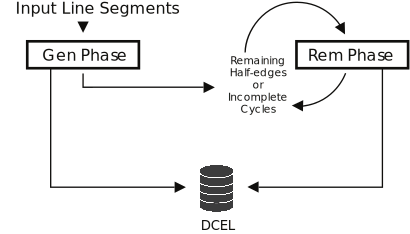
\includegraphics[width=0.75 \linewidth ]{chapterSDCEL/model/overview_updated.png}
	\caption{DCEL Constructor for Polygonization Overview}
	\label{fig:overview_ddcel}
\end{figure}

Building a DCEL data structure from an input of planar line segments extracts all closed polygons during the invocation of the \textit{polygonization} 
procedure.  In our work in \cite{abdelhafeez_ddcel_2023}, we proposed a scalable distributed framework to build a DCEL and extract polygons in parallel from 
the 
input 
line segments. Figure \ref{fig:overview_ddcel} shows an overview of the DCEL constructor. 

To create a DCEL data structure from input line segments, the \textit{DCEL constructor} undergoes a two-phase paradigm.  The \textit{Gen Phase}, detailed in 
Section \ref{sec:gen}, spatially partitions the input lines, generating the subdivision's vertices ($V$) and half-edges ($H$), and a subset of the 
subdivision's faces ($F_0$). 

The remaining line segments that are not assigned to a face yet are passed to the subsequent phase in the form of half-edges or incomplete cycles. An 
incomplete 
cycle is a connected half-edge list that is a candidate face. The \textit{Rem Phase}, detailed in Section \ref{sec:rem}, generates the subdivision's remaining 
faces, $F_j, \ \forall j > 0$. 

Section \ref{sec:partitioning_ddcel} discusses different data re-partitioning schemes with a minimal number of iterations to reduce the workload of the 
\textit{Rem Phase} without compromising correctness. The polygonization procedure produces two outputs: first, a set of closed polygons formed by the input 
planar line segments, and second, any edges that are not a part of any polygon, i.e., dangle or cut edges. Overlaying the polygons generated with any polygon 
layer follows the approaches discussed in sections \ref{sec:methods}and \ref{sec:alternative_methods}. In section \ref{sec:over_dang}, we extend the overlay 
approaches to handle overlaying a polygon layer with the remaining edges (the dangle and cut edges).

\subsection{Gen Phase}
\label{sec:gen}

The Gen phase accepts an input dataset of line segments $N$ and starts by partitioning the input across the worker nodes in a distributed cluster using a global quadtree spatial index.
Each data partition $P_i$ covers a specific spatial area represented by its minimum bounding rectangle (MBR) $B_i$.
Figure~\ref{fig:ddcel:input} shows an example of four leaf nodes of a quadtree built for input spatial line segments. Solid lines represent the line segments, and dashed lines represent the partitions' MBRs.

\begin{figure}[tb]
	\centering
	\includegraphics[width=0.75 \linewidth ]{chapterSDCEL/model/input-network}
	\caption{Partitioned input spatial lines.}
	\label{fig:ddcel:input}
\end{figure}

After spatially partitioning the input lines, each partition generates its vertices, half-edges, and faces (collectively the partition DCEL) using the subset of 
the dataset that intersects with the partition's MBR.
The \textit{partition vertices} are the vertices that are wholly contained within the partition MBR. 
On the other hand, the \textit{partition half-edges} are any half-edge that intersects with the partition MBR.
\textit{Partition faces} are the faces that are wholly contained within the MBR of the partition.
On each data partition $P_i$, the Gen phase undergoes four main procedures; 
(1) first, generating the partition vertices and half-edges, 
(2) second, marking the dangle half-edges, 
(3) third, setting the next half-edge pointers for all half-edges and marking the cut edges, 
(4) lastly, generating the partition faces. 

\vspace{4pt}
\textit{\textbf{Step 1: Generating the Partition Vertices and Half-edges.}}
\\
In the first step, the Gen Phase starts with populating the vertices and the half-edges RDDs of the DCEL data structure.
Each partition $P_i$ receives a subset of the input dataset that intersects with the partition's boundary.
For every line segment object $o$ received at partition $P_i$ ($o \in P_i$), two vertices are generated ($v_1$, $v_2$); one for each endpoint on this line 
segment ($p_1$, $p_2$). These two vertices objects ($v_1, v_2$) are appended to the vertices RDD in the DCEL data structure.
We also generate two half-edges ($h_1, h_2$) for every line segment. 
The first half-edge $h_1$ has its destination vertex $v_1$, while the other half-edge $h_2$ has its destination vertex $v_2$. These two half-edges are assigned 
as twins.
The half-edge $h_1$ is appended to the incident list of the vertex $v_1$. Similarly, $h_2$ is appended to $v_2$'s incident list.
For a half-edge to span multiple partitions, we check whether it is wholly contained within the partition MBR $B_i$; if not, and it is just intersecting, then 
this half-edge spans multiple partitions. 
These half-edges are duplicated on all partitions they intersect with.
The remaining attributes of each half-edge object are assigned in the subsequent steps. 
The two generated half-edge objects ($h_1, h_2$) are appended to the half-edges RDD in the DCEL data structure.
Figure \ref{fig:ddcel:step1} shows a graphical illustration of the DCEL data structure representing the input lines after generating the vertices and the 
half-edges on all data partitions.

\begin{figure}[tb]
	\centering
	\includegraphics[width=0.75 \linewidth ]{chapterSDCEL/model/ddcel-1}
	\caption{DCEL vertices and half-edges.}
	\label{fig:ddcel:step1}
\end{figure}


\vspace{4pt}
\textit{\textbf{Step 2: Marking the Dangle Half-edges.}}
\\
Dangle half-edges are not part of any face; thus, marking them is essential to exclude them during the polygonization procedure. To find dangles in the input 
lines, we use previously generated information, i.e., information about the vertices and their incident half-edges. 
We compute the degree of each vertex $v \in V$ populated in the previous step. A vertex degree is the number of non-dangle half-edges in its incident half-edges 
list. If the degree of an arbitrary vertex $v$ is less than or equal to 1 ($degree(v) \le 1$), then all of $v$'s incident half-edges and their twins are also 
dangle half-edges. 
Marking any new half-edge as a dangle requires recomputing the degree of the vertices connected to it. 
Thus, marking the dangle half-edges is an iterative process. After the initial run over all vertices and marking the initial dangle half-edges, we reiterate 
over the vertices to check for newly found dangle half-edges. We keep iterating until convergence when no new dangle half-edges are detected.


\vspace{4pt}
\textit{\textbf{Step 3: Setting the Half-edges' Next Pointers, and Marking the Cut Edges.}}
\\
The third step is divided into three smaller steps: (a) setting the next half-edge pointer for each half-edge, (b) marking the cut edges, and (c) updating the 
next half-edges accordingly.
To set the next pointer for each half-edge, we use information from the previous two steps, i.e., the vertices incident half-edges and the current dangle 
half-edges.
For each vertex $v \in V$, we sort its incident half-edges list in clockwise order, excluding the dangle half-edges. 
After sorting the incident half-edges list $v.incidentH$, for every pair of half-edges $v.incidentH[t]$, $v.incidentH[t+1]$ in the sorted list, we assign 
$v.incidentH[t].next$ to $v.incidentH[t+1].twin$. For the last incident half-edge in the sorted list $v.incidentH[v.incidentH.len-1]$, we assign its next 
half-edge to $v.incidentH[0].twin$.


After the initial assignment of the next half-edge pointers, we proceed with the second sub-step, marking the cut edges.
To mark the cut edges, we start our procedure at an arbitrary half-edge $h_{initial}$ and assign our $h_{current}$ half-edge pointer to it. We advance the 
$h_{current}$ pointer at each iteration to the $h_{current}$'s next ($h_{current} = h_{current}.next$), storing all visited half-edges in a list (current 
cycle). We keep advancing the $h_{current}$ pointer till we reach one of three cases.
(1) We return to the initial half-edge $h_{initial}$, which means a cycle is detected and no cut edge is detected.
(2) The half-edge $h_{current}.next$ is not available, which also means no cut edge is detected.
(3) We find $h_{current}.twin$ in the current cycle, which means that $h_{current}$ and its twin are both cut edges. 
Once we reach one of these cases, we mark all visited half-edges as such and proceed with a new arbitrary half-edge to be $h_{initial}$.
This process is terminated when all the partition half-edges are visited.

In the third sub-step, after marking all cut edges, we update the next pointers while excluding the cut edges. 
For each vertex $v \in V$, we sort its incident half-edges list in clockwise order again, now while excluding both the dangle and the cut edge half-edges.
After sorting the incident half-edges list $v.incidentH$, we re-execute the same process of the first sub-step, assigning $v.incidentH[t].next$ to 
$v.incidentH[t+1].twin$. 
Figure~\ref{fig:ddcel:step2} shows the DCEL data structure after removing the dangle and cut edges.


\begin{figure}[tb]
	\centering
	\includegraphics[width=0.75 \linewidth ]{chapterSDCEL/model/ddcel-2}
	\caption{DCEL vertices and half-edges after dangle and cut edge removal.}
	\label{fig:ddcel:step2}
\end{figure}

\vspace{4pt}
\textit{\textbf{Step 4: Generating the Partition Faces.}}
\\
Polygonization on each partition $P_i$ starts with selecting an arbitrary half-edge as our initial half-edge $h_{initial}$.
We initially assign our $h_{current}$ half-edge pointer to $h_{initial}$. We advance the $h_{current}$ pointer at each iteration to the $h_{current}$'s next 
($h_{current} = h_{current}.next$), storing all visited half-edges in a list $cycle$. We keep advancing the $h_{current}$ pointer till we reach one of the 
following cases:
(1) We return to the initial half-edge $h_{initial}$, which means that we have found a face. In this case, we add the found face $f$ to the faces collection 
$F_0$ and assign $h.incidentF = f, \;\; \forall h \in cycle$.
(2) The $h_{current}.next$ is not available, and $h_{current}$ is a half-edge that spans multiple partitions. In this case, the cycle needs more information 
from the neighboring partitions to be completed, and the current partition's data is insufficient to produce this face.
To complete this cycle, we either pass the incomplete cycle into the Rem phase (the current list $cycle$), where it collects all incomplete cycles from all 
partitions and attempts to join them to form a face. Another approach would be passing the plain half-edges in this cycle to the next phase. Both approaches are 
discussed in detail in Section~\ref{sec:rem}.
Once we finish processing this cycle, we mark all visited half-edges as such, clear the cycle, and proceed with a new arbitrary half-edge to be $h_{initial}$.
This process is terminated when all the partition half-edges are visited.
In Figure~\ref{fig:ddcel:faces}, the dotted faces are the faces generated in this phase (Gen Phase).

\begin{figure}[tb]
	\centering
	\includegraphics[width=0.75 \linewidth ]{chapterSDCEL/model/ddcel-3}
	\caption{DCEL faces.}
	\label{fig:ddcel:faces}
\end{figure}

\subsection{Rem Phase}
\label{sec:rem}

The Rem Phase accepts the remaining half-edges or incomplete cycles as input. 
To be included in the remaining half-edges set, a half-edge cannot be a dangle or a cut edge. Also, the half-edge should not have been bounded to a face yet.
An incomplete cycle is a sequence of half-edges that acts as a candidate face. This incomplete cycle could not be completed since their marginal half-edges span multiple partitions.


The Rem Phase is an iterative phase, where each iteration $j$ generates a subset of faces $F_j$. The unused input data at iteration $j$ is passed to the next iteration $j+1$.
Faces generated from the Gen phase and the Rem phase constitute the whole faces of the subdivision $F$.
In each iteration, the Rem Phase starts with re-partitioning the input data across the worker nodes using a new set of partitions.
This new set of partitions satisfies the convergence criteria; the new number of partitions ($k_j$) at iteration $j$ must be less than the number of partitions ($k_{j-1}$) at iteration $j-1$. This criterion ($k_j < k_{j-1}$) ensures there is an iteration ($m$) at which the remaining line segments are re-partitioned to one partition only, where $m$ is the total number of iterations of the Rem Phase, converging the problem into a sequential one and guaranteeing the termination of the procedure.
After the data re-partitioning, we proceed with generating a subset of the remaining faces. Two approaches are employed for the remaining faces generation, depending on the phase input data.
The first approach assumes the phase input is a set of the \underline{R}emaining \underline{H}alf-edges (RH Approach). 
While the second approach assumes the input is a set of the \underline{I}ncomplete \underline{C}ycles (IC Approach). 

\vspace{4pt}
\textit{\textbf{RH Approach: Iterate over the Remaining Half-edges.}}
\\
At each iteration $j$ and on each new data partition, a subset of the remaining half-edges is received. 
Duplicate half-edges received on one new partition are merged into a single half-edge choosing the half-edge with the available next half-edge.
We follow the same procedure of generating faces in the Gen Phase. Starting from an arbitrary half-edge as our initial half-edge $h_{initial}$, we assign our $h_{current}$ half-edge pointer initially to $h_{initial}$. We advance the $h_{current}$ pointer at each iteration to the $h_{current}$'s next ($h_{current} = h_{current}.next$), storing all visited half-edges in a list $cycle$. We keep advancing the $h_{current}$ pointer till we reach one of the following cases:
(1) We return to the initial half-edge $h_{initial}$, which means that we have found a face. In this case, we add the found face $f$ to the faces collection $F_j$ and assign $h.incidentF = f, \;\; \forall h \in cycle$.
(2) The $h_{current}.next$ is not available, and $h_{current}$ is a half-edge that is not wholly contained in the new partition MBR.
Once we finish processing this cycle, we mark all visited half-edges as such, clear the cycle, and proceed with a new arbitrary half-edge to be $h_{initial}$.
This iteration is terminated when all the remaining half-edges are visited. All half-edges that have not been assigned to any face yet are passed to the next iteration.
The Rem Phase terminates if (1) there are no more remaining half-edges, i.e., all non-dangle non-cut edge half-edges are assigned to a face, or (2) the remaining half-edges have been processed on one partition.

\vspace{4pt}
\textit{\textbf{IC Approach: Iterate over the Incomplete Cycles.}}
\\
At each iteration $j$, and on each new data partition, a subset of the incomplete cycles is received. 
Starting from an arbitrary incomplete cycle $c_{initial}$ with first half-edge $first(c_{initial})$ and last half-edge $last(c_{initial})$, where the first and last half-edges are the incomplete cycle's terminal half-edges, we search for a match $c_{match}$ in the remaining incomplete cycles such that the $last(c_{initial}) = first(c_{match})$. When a match is found, we merge the two cycles such that the $last(c_{initial})$ is now the $last(c_{match})$. We keep merging cycles till we reach one of the following cases:
(1) The $last(c_{match}) = first(c_{initial})$, which means the cycle is now completed. In this case, we add the found face $f$ to the faces collection $F_j$ and remove all incomplete cycles used from the set of the incomplete cycles.
(2) We can not find a match for the current last half-edge, and the last half-edge is not wholly contained within the new partition's MBR. In this case, the incomplete cycle needs more information from the neighboring partitions to be completed, and the current partition's data is insufficient to produce this face.
Once we finish processing this matching process, we mark all visited incomplete cycles as such and proceed with a new arbitrary incomplete cycle to be $c_{initial}$.
This iteration $j$ is terminated when all the incomplete cycles are visited. All incomplete cycles that are not completed yet are passed into the next iteration.
The Rem Phase terminates if (1) there are no more remaining incomplete cycles, i.e., all cycles have been completed, or (2) the incomplete cycles have been processed on one partition.
In Figure \ref{fig:ddcel:faces}, the hatched faces are the faces generated in the first iteration ($j=1$) of the Rem Phase.


\subsection{Data Partitioning}\label{sec:partitioning_ddcel}

The quadtree partitioner is used again to distribute the data amongst the worker nodes across the cluster. In the Gen Phase, the quadtree leaf nodes are used as the initial data partitions.
The output of the Gen Phase, whether the remaining half-edges or the incomplete cycles, is iteratively re-partitioned into new sets of partitions.
Each iteration set of partitions must satisfy the convergence criterion to ensure that the Rem Phase will terminate.
We employ the same quadtree partitioner to generate the new partitions. 
Assume we have a quadtree built on the input line segments of height $L$. 
At the Gen Phase, we use nodes at the leaf level $L$ as our initial data partitions. For each iteration $j$ in the Rem Phase, we level up in the quadtree and choose different level nodes, aside from the leaves, to be our current data partitions.  
We keep leveling up in the quadtree till we reach the root ($l=0$), which means that all data is located on only one partition (the root).
Going up in the quadtree ensures that the number of partitions at iteration $j+1$ is less than that at iteration $j$ since the number of nodes at any arbitrary level $l$ visited at iteration $j$ is more than that at level $l_{chosen}, \ \forall l_{chosen} < l$ visited at iteration $j+1$.


We always start with the leaf nodes level $L$ in the Gen Phase. Choosing which levels to visit next in each iteration $j$ is a system parameter. 
We offer different schemes for the visited quadtree levels: 
\begin{enumerate}
    \item Going directly to the root node at $l=0$ after the leaf nodes, i.e., visiting only levels L in the Gen and 0 in the Rem phases. However, the experimental evaluation shows that collecting the data after the Gen phase on one node is prohibitive, and one worker node will not be able to process the Gen phase's output.
    \item Going \underline{1} \underline{L}evel \underline{U}p (1LU) each iteration, i.e. if we visit level $l$ at iteration $j$, we go to level $l-1$ at iteration $j+1$. This means the Rem Phase visits all the quadtree levels resulting in $L$ iterations.
    \item Going \underline{2} \underline{L}evels \underline{U}p (2LU) each iteration resulting in half the number of iterations $\frac{L}{2}$ compared to 1LU.
    \item Skipping to the \underline{M}iddle of the tree at level $\frac{L}{2}$, then continue going 1 level up for the remaining levels (M1LU), which will also result in $\frac{L}{2}$ iterations.
    \item Skipping to the \underline{M}iddle of the tree every time, dividing the current level by two each iteration (MU); this will result in $\log_2(L)$ iterations.
\end{enumerate}
The goal is to find a re-partitioning scheme with a minimal number of iterations, thus reducing the workload of the Rem Phase while ensuring that the worker nodes can process the chunk of the data it receives at each iteration $j$.
The extreme case of having only one iteration at the Rem Phase will not work since the data is too big to fit one partition and be processed by only one worker node. On the other hand, the more unnecessary iterations we have, the more overhead on the system resulting in higher query latency.


\subsection{Overlaying Polygons with Dangle and Cut Edges} \label{sec:over_dang}

\begin{figure}[tb]
	\centering
	\includegraphics[width=0.75 \linewidth ]{chapterSDCEL/model/DangleOverlay1.pdf}
	\caption{Spatial partitioning of input layers A and B}
	\label{fig:dangleoverlay:input}
\end{figure}

\begin{figure}[tb]
	\centering
	\includegraphics[width=0.75 \linewidth ]{chapterSDCEL/model/DangleOverlay2.pdf}
	\caption{Re-Partitioning of polygon $A_0$ with edges it intersects with}
	\label{fig:dangleoverlay:inter}
\end{figure}

\begin{figure}[tb]
	\centering
	\includegraphics[width=0.75 \linewidth ]{chapterSDCEL/model/DangleOverlay3.pdf}
	\caption{The result of polygonization of $A_0$ with $B_0, B_1, B_2$}
	\label{fig:dangleoverlay:result}
\end{figure}

The polygonization procedure produces two outputs: first, a set of closed polygons formed by the input planar line segments, and second, any edges that are not 
a part of any polygon, i.e., dangle or cut edges. 
Overlaying the polygons generated with any polygon layer follows the approaches discussed in sections \ref{sec:methods} and \ref{sec:alternative_methods}.
However, we need to modify the algorithms provided in these previous sections to overlay an input polygon layer $A$ with the dangle and cut edges, i.e. layer 
$B$. In particular, we modify the reduce phase.
Figure \ref{fig:dangleoverlay:input} illustrates the spatial partitioning of the two input layers, $A$ and $B$. Layer $A$ contains two input polygons, $A_0$ and 
$A_1$, while Layer $B$ consists of three dangle edges, $B_0$, $B_1$, and $B_2$.

Each edge from layer $B$ is labeled a unique label and is fed as an input to the overlay module.
The local overlay is performed by finding intersections between the input polygon layer $A$ and layer $B$ on each data partition.
If a polygon with $id = i$ from polygon layer $A$ intersects with edges with ids $id = a, id = b, id = c$ from layer $B$ at some data partition, we generate a 
label to match these intersections $A_{i} B_{a} B_{b} B_{c}$. 
At the reduce phase, we re-partition the data by the first label, meaning we collect all edges that intersect with the first label.
If two data partitions produced the labels $A_{i} B_{a} B_{b} B_{c}$ and $A_{i} B_{x} B_{y}$, we repartition the data such that $A_{i}$ is on one partition with 
all edges it is intersecting, i.e., $B_{a}, B_{b}, B_{c}, B_{x}, B_{y}$.
In Figure \ref{fig:dangleoverlay:inter}, Polygon $A_0$ is re-partitioned along with the edges it intersects, specifically $B_0$, $B_1$, and $B_2$.

After re-partitioning the data, we have all edges from both layers intersecting each other on the same partition. The next step is to find the polygons 
generated by these intersections. Since there is no guarantee that only one polygon is generated, we substitute the polygon concatenation proposed in 
Section~\ref{sec:reduce} by performing \textit{polygonization} on each partition. The polygonization procedure ensures it generates all new possible polygons. 
The polygonization procedure follows the algorithm mentioned in Section~\ref{sec:gen}. It starts with generating the new vertices and half-edges, then marking 
the current dangles and cut edges, then setting the next pointers and finally generating the partition polygons.
Figure \ref{fig:dangleoverlay:result} shows the result of polygonizing the edges from Polygon $A_0$ and $B_0$, $B_1$, and $B_2$, resulting in two polygons, 
$A_01$ and $A_02$.

Polygons from all partitions generate the overlay between the polygon layer $A$ and layer $B$.

\section{Experimental Evaluation} \label{sec:extension_experiments}

\subsection{Kd-tree versus quadtree performance} \label{sec:comparison}
To compare the quadtree and kd-tree partition strategies, we analyze their performance across several stages: constructing the spatial data structure to define the partition cells based on the sample, the cost of partitioning, populating the cells with the full datasets, and the overall time required to complete each phase of the overlay operation using each partitioning approach. We use the MainUS and GADM datasets, as described in Table \ref{tab:datasets}.

 \begin{figure}
    \centering
    \includegraphics[width=\textwidth]{chapterExtension/K/K_Creation}
    \caption{Construction time for the spatial data structure in the (a) MainUS and (b) GADM datasets.}\label{fig:k_creation_us}
 \end{figure}

Figure \ref{fig:k_creation_us} illustrates the construction time for sampling the input layers and generating partitioning cells with varying numbers of divisions. The kd-tree requires more time, primarily due to the sorting involved at each split to organize the data and locate the midpoint. On average, the quadtree takes only 23.13\% of the time needed to create the kd-tree (21.55\% for MainUS and 24.72\% for GADM). However, kd-tree creation accounts for only 5.86\% of the total time required for complete DCEL construction (6.88\% for MainUS and 4.87\% for GADM).

 \begin{figure}
    \centering
    \includegraphics[width=\textwidth]{chapterExtension/K/K_Space} 
    \caption{Number of cells created by each spatial data structure in the (a) MainUS and (b) GADM datasets.} \label{fig:k_space_us}
 \end{figure}

 An important characteristic of each partitioning scheme is the number of cells (partitions) generated by each sample data structure. Figure \ref{fig:k_space_us} shows the number of cells created by each spatial data structure. Since the quadtree follows a space-oriented technique, it creates more nodes (four at each split), resulting in a larger number of leaf cells, many of which are likely to be empty compared to those generated by the kd-tree.

 \begin{figure}
    \centering
    \includegraphics[width=\textwidth]{chapterExtension/K/K_Partitioning} 
    \caption{Data partitioning time using a spatial data structure (a) in the MainUS dataset and (b) in the GADM dataset.} \label{fig:k_partitioning_us}
 \end{figure}

 Figure \ref{fig:k_partitioning_us} presents the cost of partitioning the full content of both layers. Based on the sample tree data structure, each edge is assigned to a cell (partition) according to the leaf in which it is located; edges are assigned (or duplicated) to all leaves they intersect. A shuffle operation is then performed to move the data to the corresponding node responsible for handling each cell (partition). The figure shows that quadtree partitioning takes more time, primarily due to the larger number of leaves generated by the sample tree and the higher number of edges overlapping multiple partitions, which is expected with the quadtree’s use of smaller, more numerous cells.

\begin{figure}
    \centering
    \includegraphics[width=\textwidth]{chapterExtension/K/K_Overlay} 
    \caption{Execution time for the overlay operation using a spatial data structure in the MainUS (a)and GADM (b) dataset.} \label{fig:k_overlay_us}
\end{figure}

Once the data is assigned to their respective partitions, the overlay operation can be executed.  Figure \ref{fig:k_overlay_us} illustrates the overlay performance for each partitioning strategy with varying numbers of cells. The kd-tree approach performs better, as the quadtree’s tendency to generate a higher number of empty cells negatively impacts its performance.

\begin{figure}
    \centering
    \includegraphics[width=\textwidth]{chapterExtension/K_SS/K_SS}
    \caption{(a)Speed Up and (b) Scale Up performance of the Kdtree partitioning using the MainUS dataset.} \label{fig:k_scale_speed_us}
\end{figure}

Finally, we evaluate the speed-up and scale-up performance of the kd-tree partitioning. Figure \ref{fig:k_scale_speed_us}(a) presents the speed-up performance for the MainUS dataset (36 million edges) as the number of nodes varies (3, 6, and 12 nodes). Similar to the quadtree partitioning strategy, the kd-tree partitioning demonstrates strong speed-up performance. Doubling the resources nearly halves the execution time, indicating effective scalability.

Figure \ref{fig:k_scale_speed_us}(b) illustrates the scale-up performance of the kd-tree partitioning approach. Following the procedure outlined in Section \ref{sec:speed_scale}, we generated datasets with 8M, 16M, and 32M edges from the MainUS dataset and applied the kd-tree partitioning strategy using 3, 6, and 12 nodes, respectively. The kd-tree partitioning demonstrates strong scale-up performance, maintaining consistent speed-up as the load per node remains nearly equal.

\subsection{Overlaying Polygons with Dangle and Cut Edges}

\begin{table}
    \small
    \caption{Overlaying Polygons with Dangle and Cut Edges Dataset}
    \label{tab:dangles}
    \begin{tabular}{c c c c}
        \toprule
        Dataset & Number Layer $A$ of Polygons & Number of Layer $B$ Edges & Result Polygons \\
        \midrule
        TN & 1,272 & 3,380,780 & 41,761 \\
        GA & 1,633 & 4,647,171 & 49,125 \\
        NC & 1,272 & 7,212,604 & 22,413 \\
        TX & 4,399  & 8,682,950 & 98,635 \\
        VA & 1,554 & 8,977,361 & 38,941 \\
        CA & 7,038 & 9,103,610 & 96,916\\
        \bottomrule
    \end{tabular}
\end{table}

\begin{figure}
    \centering
    \includegraphics[width=0.6\textwidth]{chapterExtension/states.pdf}
    \caption{Overlaying State polygons with dangle and cut edges.}
    \label{fig:dangle}
\end{figure}

In this section, we examine the performance of overlaying polygons with dangle and cut edges resulting from the polygonization process, as detailed in \ref{sec:over_dang}.  Table \ref{tab:dangles} presents the number of polygons per state for the first overlay layer, the number of dangle and cut edges per state for the second overlay layer, and the number of resulting polygons per state.

From Figure \ref{fig:dangle}shows that the running time is influenced by both the number of dangle and cut edges and the number of intersections between the two layers (indicated by the number of generated polygons). TN and GA have relatively fewer dangle and cut edges, leading to lower execution times compared to VA, TX, and CA. However, because NC has significantly fewer intersections than TN and GA, it exhibits the lowest execution time overall. While TX, VA, and CA have a comparable number of edges, VA’s lower number of intersections results in a shorter execution time compared to TX and CA.

\section{Conclusions} \label{sec:conclusions}
We introduced SDCEL, a scalable approach to compute the overlay operation among two layers that represent polygons from a planar subdivision of a surface. Both input layers use the DCEL edge-list data structure to store their polygons. We support input polygons in clean polygon format and polygons represented by scattered line segments through scalable polygonization. Existing sequential DCEL overlay implementations fail for large datasets. We first presented two partition strategies that guarantee that each partition collects the required data from each layer to work independently. We also proposed several optimizations to improve performance. Our experimental evaluation using real datasets shows that SDCEL has very good scale-up and speed-up performance and can compute the overlay over very large layers (up to 37M edges) in a few seconds.

\backmatter

\bmhead{Acknowledgements}
We would like to thank Sergio Rey from the Center for Geospatial Sciences for introducing us to the Scalable DCEL problem.

\section*{Declarations}

\begin{itemize}
\item Funding: This work was partially supported by the National Science Foundation under grants IIS-1901379, IIS-2237348, CNS-2031418, SES-1831615 and the Google-CAHSI research grant. 
\item Data availability: Data description and access is described in the experimental section.  The sources of the dataset are publicly available and the references and cited accordingly.
\end{itemize}


%%===========================================================================================%%
%% If you are submitting to one of the Nature Portfolio journals, using the eJP submission   %%
%% system, please include the references within the manuscript file itself. You may do this  %%
%% by copying the reference list from your .bbl file, paste it into the main manuscript .tex %%
%% file, and delete the associated \verb+\bibliography+ commands.                            %%
%%===========================================================================================%%

\bibliography{sdcel,ddcel-references}% common bib file
%% if required, the content of .bbl file can be included here once bbl is generated
%%\input sn-article.bbl

\end{document}
